\section{Membrane}
\label{sec:membrane}

\begin{frame}
    \frametitle{Molecular abstraction}
    
    \begin{itemize}
        \item Molecule class allows future extensions to different molecules and potentials
        \item Has own intra-molecular forces using \texttt{calculateIntraMolecularForces} method
        \item Molecule class offers \texttt{generateMolecule} method to construct the molecule
    \end{itemize}

    \vspace{7pt}
    \hrule

    \begin{columns}
        \begin{column}{0.6\textwidth}
            \begin{itemize}
                \item Membrane class inherits from molecule class
                \item A membrane is generated as a cuboid cluster
                \item Introduced a unique ID attribute for particles (which is their index within the particle cluster)
                \item[] \!\!\!\!\!\!\!\!\! \textcolor{orange}{$\Rightarrow$} Allowed us to store only the molecular IDs in the neighbor maps
                \item By storing only half of the neighbors we enabled parallel force calculations by using Newton's third law (stencil)
                \item The Membrane takes care of its own forces and must only be disregarded in the other force calculations
            \end{itemize}
        \end{column}
        \begin{column}{0.4\textwidth}
            \begin{figure}
                \centering
                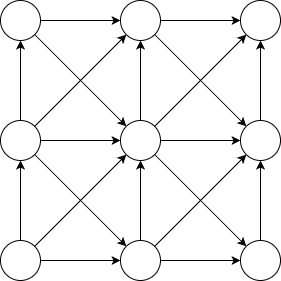
\includegraphics[width=0.6\columnwidth]{../../res/membraneNeighbor.drawio}
                \caption{Neighborhood of particles. Results in directed non-cyclic graph.}
                \label{fig:mem}
            \end{figure}
        \end{column}
    \end{columns}

    
\end{frame}